% Created 2025-03-18 ter 14:37
% Intended LaTeX compiler: lualatex
\documentclass{beamer}
\usetheme{default}
\author{fabio}
\date{\today}
\title{}
\hypersetup{
 pdfauthor={fabio},
 pdftitle={},
 pdfkeywords={},
 pdfsubject={},
 pdfcreator={Emacs 30.1 (Org mode 9.7.11)}, 
 pdflang={English}}
\begin{document}

\begin{frame}{Sumário}
\tableofcontents
\end{frame}

\begin{frame}[label={sec:orgd9c8d62}]{Separação de Misturas}
\begin{block}{Misturas homogêneas}
As misturas homogêneas apresentam-se de forma uniforme, em apenas uma fase (monofásica). Um bom exemplo de sistema homogêneo é a mistura da água e açúcar.

\begin{center}
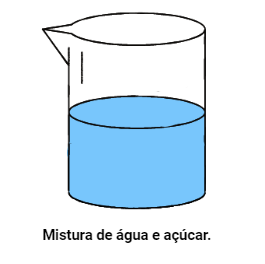
\includegraphics[scale=0.5]{../img/homogenea.png}
\end{center}
\end{block}
\begin{block}{Separação de misturas heterogêneas}
As misturas heterogêneas são aquelas constituídas por duas ou mais substâncias, que podem ser visualmente distinguíveis em um microscópio óptico. Nesse tipo de mistura os componentes ficam em fases diferentes. Um bom exemplo de sistema heterogêneo é a mistura da água e do óleo.

\begin{center}
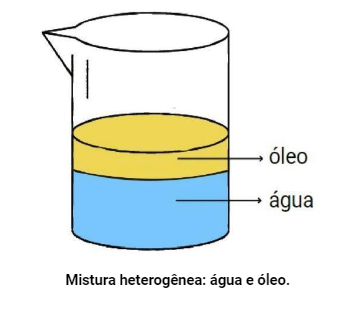
\includegraphics[scale=0.5]{../img/heterogenea.png}
\end{center}
\end{block}
\begin{block}{Misturas Heterogêneas}
\begin{columns}
\begin{column}{0.48\columnwidth}
\begin{block}{}
\begin{itemize}
\item Decantação
\item Centrifugação
\item Sifonação
\item Catação
\item Ventilação
\item Filtração
\item Peneiração
\item Dissolução fracionada
\end{itemize}
\end{block}
\end{column}
\begin{column}{0.48\columnwidth}
\begin{block}<2->{}
\begin{itemize}
\item Flotação
\item Separação magnética
\item Levigação
\item Cristalização fracionada
\item Sublimação
\item Destilação
\item Destilação fracionada
\item Cromatografia
\end{itemize}
\note{This will be formatted as a beamer note
}
\end{block}
\end{column}
\end{columns}
\end{block}
\end{frame}
\begin{frame}[label={sec:orgc09ae4c}]{Decantação}
\begin{block}{Decantação}
Usada na separação de misturas heterogêneas de solido/líquido ou de dois líquidos imiscíveis entre si.


\begin{center}
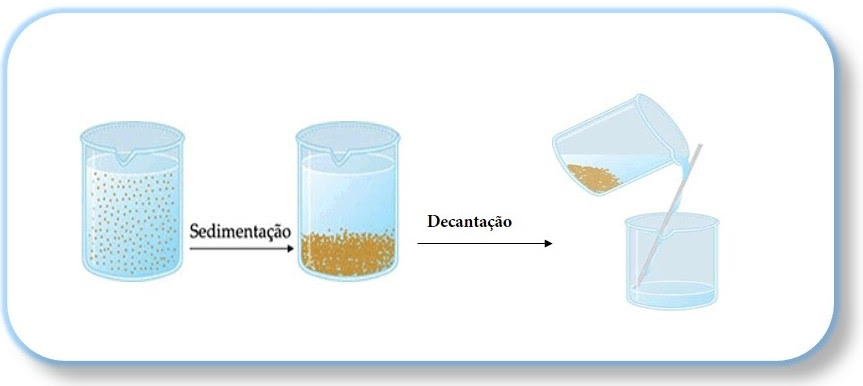
\includegraphics[width=.9\linewidth]{../img/decantacao.jpg}
\end{center}
\end{block}
\begin{block}{Funil de Separação}
Para se separar misturas heterogêneas líquido/líquido pode se utilizar também um aparelho de vidro chamado, funil de separação ou funil de decantação, funil de bromo. 

Após a decantação, abre-se cuidadosamente a torneira, deixando passar primeiro o líquido mais denso, e depois o menos denso, separando-os.

\begin{center}
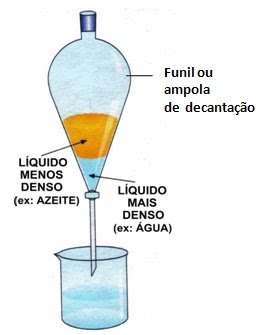
\includegraphics[scale=0.5]{../img/decantação.jpg}
\end{center}
\end{block}
\end{frame}
\begin{frame}[label={sec:org0e7f115}]{Centrifugação}
\begin{block}{Centrifugação}
Caso a decantação de uma mistura heterogênea seja muito lenta, pode-se utilizar uma alternativa mais rápida, a centrifugação. A centrifugação ocorre em um aparelho chamado \alert{centrífuga}.

A centrifugação consiste em submeter a mistura a uma rotação, onde a parte mais densa se deposita no fundo e a menos densa na parte superior.

\begin{center}
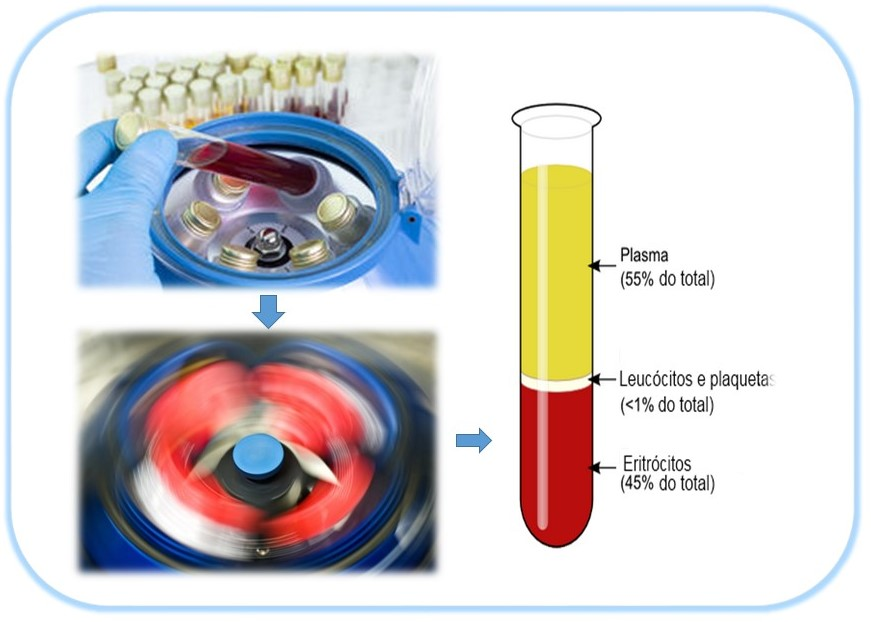
\includegraphics[scale=0.3]{../img/centrifugacao.jpg}
\end{center}
\end{block}
\end{frame}
\begin{frame}[label={sec:orge3c27ca}]{Sifonação}
\begin{block}{Sifonação}
Esse método parte da decantação. Quando a mistura é deixada em repouso, após a separação das duas fases, se não for possível retirar o líquido para o outro recipiente, podemos retirá-lo por sifonação, através de um sifão, da sucção e da ação gravitacional.

Usado para separar: \alert{sólido + líquido} ou \alert{líquido + líquido}.

Exemplo: Água + cascalho.

\begin{center}
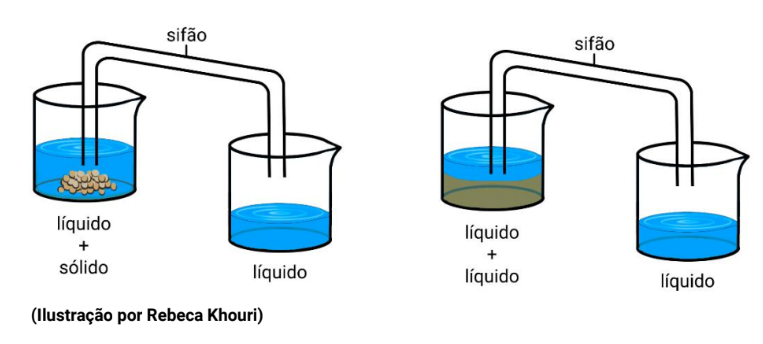
\includegraphics[scale=0.6]{../img/sifonacao.png}
\end{center}
\end{block}
\end{frame}
\begin{frame}[label={sec:orge0d5fd0}]{Catação}
\begin{block}{Catação}
A catação é um método de separação de misturas heterogêneas manualmente, utilizando apenas a mão ou tendo como auxílio algum instrumento, geralmente uma colher ou uma pinça.

Nesse processo, que separa substâncias sólidas de outras substâncias também sólidas (sólido + sólido), para remover as partículas de uma mistura é necessário que elas.

\begin{itemize}
\item Sejam visíveis a olho nu;
\item Estejam em pequenas quantidades;
\item possam ser distinguidas na mistura por cor, tamanho ou formato.
\end{itemize}
\begin{center}
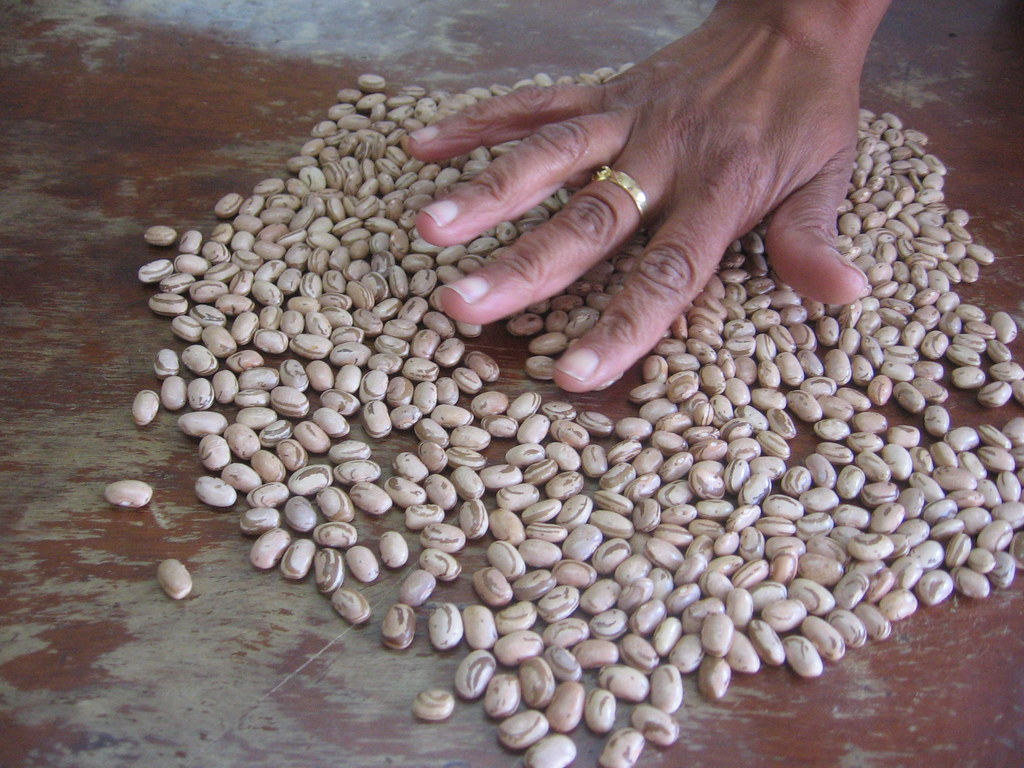
\includegraphics[width=.9\linewidth]{../img/catacao.jpg}
\end{center}
\end{block}
\end{frame}
\begin{frame}[label={sec:org5d62291}]{Ventilação}
\begin{block}{Ventilação}
\alert{Ventilação} é um processo físico de separação de misturas heterogêneas. Que é utilizado quando os sólidos granulados que formaram a mistura possuem densidades sensivelmente diferentes. Nesse caso, passa-se uma forte corrente de ar pela mistura e o menos denso é arrastado pelo vento e separado dos mais densos.

\begin{center}
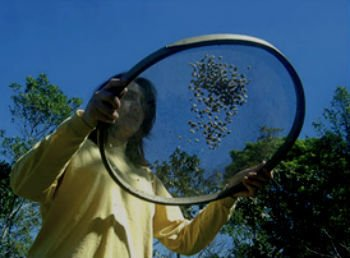
\includegraphics[scale=0.5]{../img/ventila.jpg}
\end{center}
\end{block}
\end{frame}
\begin{frame}[label={sec:org88c2a08}]{Evaporação}
\begin{block}{Evaporação}
Na separação de misturas homogêneas pode se empregar a técnica da evaporação. É um processo barato, e utilizado quando só há interesse na fase sólida.
A técnica consiste na evaporação da fase líquida, retendo somente a fase sólida. Muito utilizada na separação do sal da água do mar.

\begin{center}
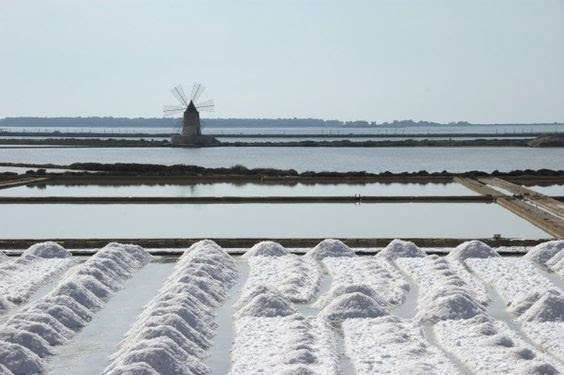
\includegraphics[scale=0.5]{../img/evaporacao_sal.jpg}
\end{center}
\end{block}
\end{frame}
\begin{frame}[label={sec:org6152427}]{Filtração}
\begin{block}{Filtração}
A filtração é um método físico de separação de misturas heterogêneas, quando temos um sólido disperso em um líquido ou gás. Basicamente, passa-se a mistura heterogênea por um filtro, isto é, um material poroso, no qual ficam retidas as partículas sólidas suspensas, a parte líquida ou gasosa atravessa o filtro.

\begin{itemize}
\item \alert{Filtração Simples}
\item \alert{Filtração à vácuo}
\end{itemize}
\end{block}
\begin{block}{Filtração Simples}
Usa-se um papel de filtro convenientemente dobrado em quatro, formando um cone, como na imagem abaixo:


\begin{center}
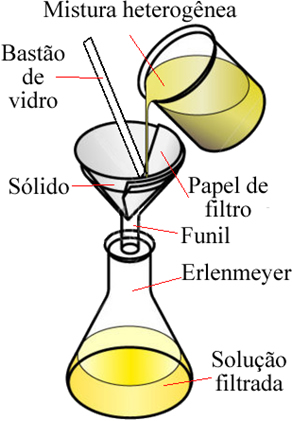
\includegraphics[scale=0.5]{../img/filtracao.jpg}
\end{center}
\end{block}
\begin{block}{Filtração à vácuo}
Filtração a vácuo: Quando uma filtração é muito demorada, pode-se realizar a filtração a vácuo, também chamada de filtração por pressão reduzida, que acelera o processo.

Em laboratório, esse tipo de filtração é realizado usando-se um funil de Buchner feito de porcelana que tem o fundo perfurado.

\begin{center}
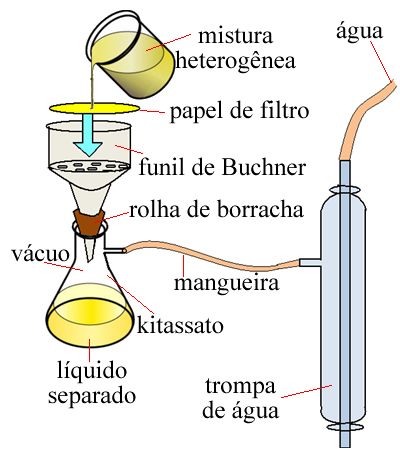
\includegraphics[scale=0.4]{../img/filtracao-a-vacuo.jpg}
\end{center}
\end{block}
\end{frame}
\begin{frame}[label={sec:org31c4963}]{Peneiração}
\begin{block}{Peneiração}
A peneiração ou tamisação consiste em peneirar as substâncias para separar os componentes sólidos. A mais grossa fica retida na peneira à medida que a mais fina passa pelos furinhos do utensílio.

\begin{center}
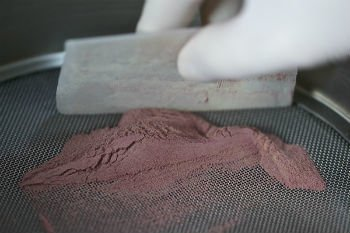
\includegraphics[scale=0.4]{../img/peneiracao.jpg}
\end{center}
\end{block}
\end{frame}
\begin{frame}[label={sec:org9a944fa}]{Dissolução fracionada}
\begin{block}{Dissolução fracionada}
Dos muitos métodos que existem para separar misturas heterogêneas de dois ou mais sólidos, um deles é a dissolução fracionada. Essa técnica de separação está baseada na diferença de facilidade com que os os sólidos componentes de uma mistura dissolvem-se em determinado solvente.

A dissolução fracionada é aplicada quando se tem uma mistura de sólidos em que apenas um desses componentes é solúvel em um determinado líquido. Um exemplo de mistura, onde se é possível aplicar essa técnica, é uma mistura de açúcar e areia, ao adicionarmos água, apenas o açúcar irá se dissolver.

\begin{center}
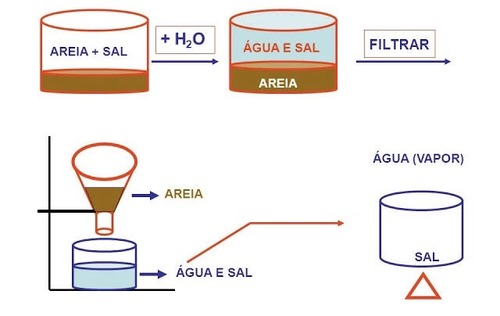
\includegraphics[scale=0.3]{../img/dissolucao.jpg}
\end{center}
\end{block}
\end{frame}
\begin{frame}[label={sec:org0d48604}]{Flotação}
\begin{block}{Flotação}
A flotação é um tipo de processo físico de separação de misturas heterogêneas. Essa técnica consiste em adicionar bolhas de ar ao meio para que as partículas em suspensão no líquido aglutinem-se a essas bolhas.

\begin{center}
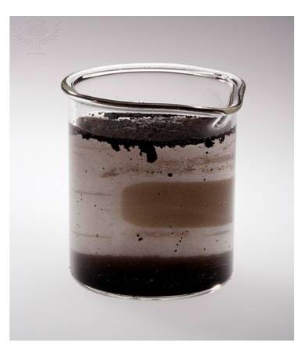
\includegraphics[scale=0.4]{../img/flotacao.png}
\end{center}
\end{block}
\end{frame}
\begin{frame}[label={sec:orgec54a50}]{Separação magnética}
\begin{block}{Separação magnética}
A separação magnética é um método de separação de misturas heterogêneas de componentes sólidos, mais especificamente para separação de misturas contendo ferro magnético como o cobalto, o níquel e, principalmente, o ferro.

\begin{center}
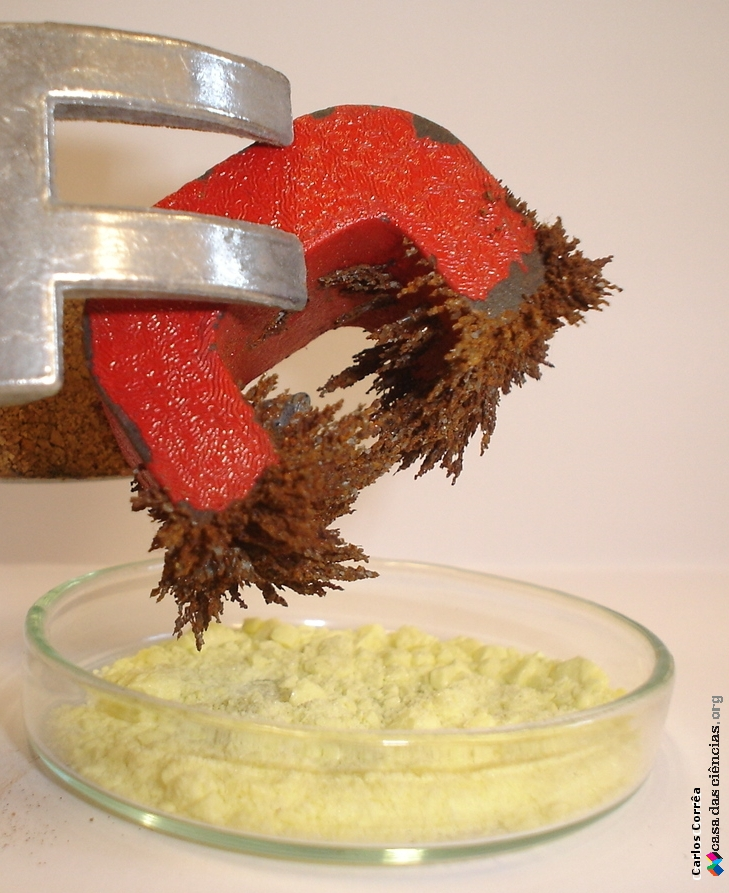
\includegraphics[scale=0.2]{../img/separacao_magnetica.jpg}
\end{center}
\end{block}
\end{frame}
\begin{frame}[label={sec:org2577478}]{Levigação}
\begin{block}{Levigação}
Neste método, um dos sólidos da mistura possui menor densidade e pode ser carregado pela água corrente. Os garimpeiros costumam separar o ouro da areia dessa forma, pois quando passam a água corrente pela mistura, a areia, que é menos densa, é arrastada e o ouro, que é mais denso, permanece no fundo do recipiente que eles usam, que é denominado de bateia

\begin{center}
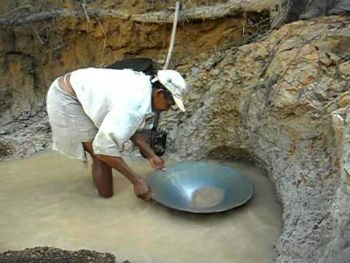
\includegraphics[scale=0.5]{../img/levigacao.jpg}
\end{center}
\end{block}
\end{frame}
\begin{frame}[label={sec:org8739c44}]{Cristalização fracionada}
\begin{block}{Cristalização fracionada}
A cristalização fracionada é um processo de separação de misturas, onde as substâncias da mistura são sólidas. Dissolvendo todos os componentes da mistura em líquido, que logo em seguida sofre evaporação, ele provoca a cristalização das substâncias separadamente.

\begin{center}
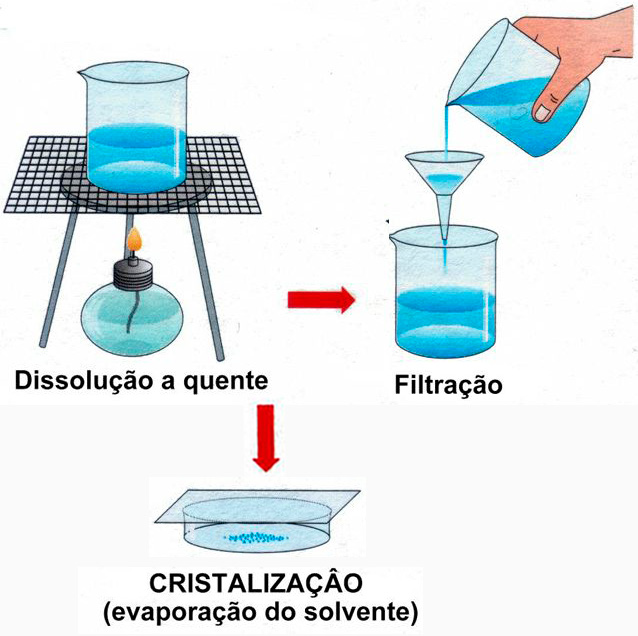
\includegraphics[scale=0.2]{../img/cristalizacao_fracionada.png}
\end{center}
\end{block}
\end{frame}
\begin{frame}[label={sec:org4048b54}]{Floculação}
\begin{block}{Floculação}
É um processo de separação de misturas utilizado no tratamento da água para abastecimento público. O processo físico promove a aglutinação das partículas já coaguladas, facilitando o choque entre as mesmas devido à agitação lenta. A formação de flocos de impurezas facilita sua posterior remoção por sedimentação sob ação da gravidade, flotação ou filtração.

\begin{center}
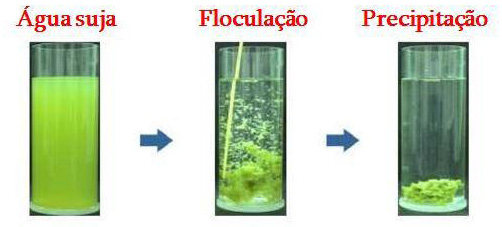
\includegraphics[scale=0.6]{../img/floculacao.png}
\end{center}
\end{block}
\end{frame}
\begin{frame}[label={sec:org64f129d}]{Sublimação}
\begin{block}{Sublimação}
Técnica que permite separar uma substância sólida que sublime facilmente (um exemplo é o iodo como mostra a imagem) de outras com menos facilidade em sublimação.

\begin{center}
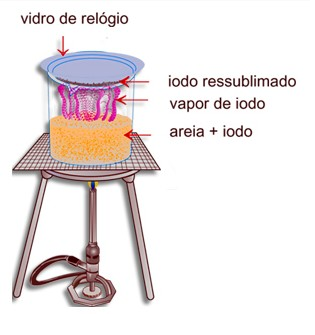
\includegraphics[scale=0.5]{../img/sublimacao.png}
\end{center}
\end{block}
\end{frame}
\begin{frame}[label={sec:orge5cbe24}]{Destilação}
\begin{block}{Destilação Simples}
Usada em separação  de mistura homogênea sólido/líquido quando há interesse tanto na fase líquida quanto na fase sólida. A separação da substâncias ocorre pela diferença nos pontos de ebulição.

\begin{center}
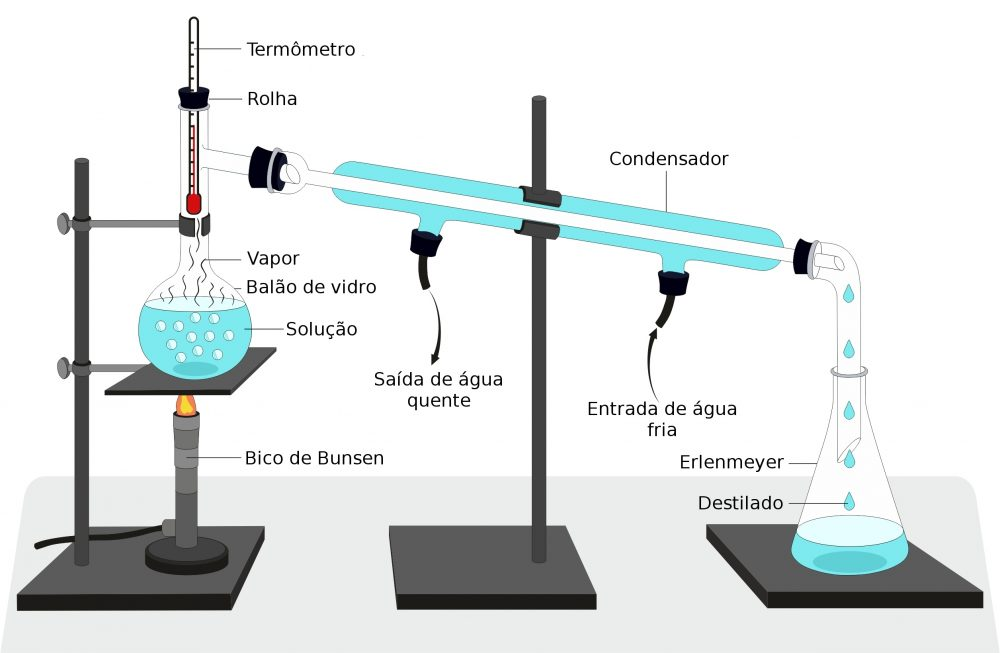
\includegraphics[scale=0.3]{../img/destilacao-simples.jpg}
\end{center}
\end{block}
\begin{block}{Destilação Fracionada}
Para misturas homogêneas de dois ou mais líquidos, utiliza-se a técnica da destilação fracionada. Assim como na destilação simples, a técnica é baseada na diferença dos pontos de ebulição das substâncias ali presente. 

\begin{center}
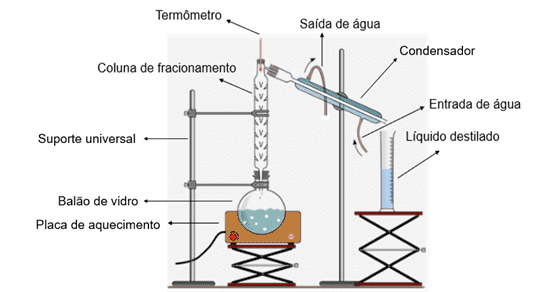
\includegraphics[scale=0.5]{../img/destilacao-fracionada.png}
\end{center}
\end{block}
\begin{block}{Destilação do Petróleo}
Processo utilizado na separação dos componentes do petróleo. Essa técnica também é empregada para a separação de gases na atmosfera. Onde o ar é resfriado até atingir o estado líquido e a seguir passa por \alert{destilação fracionada}.

\begin{center}
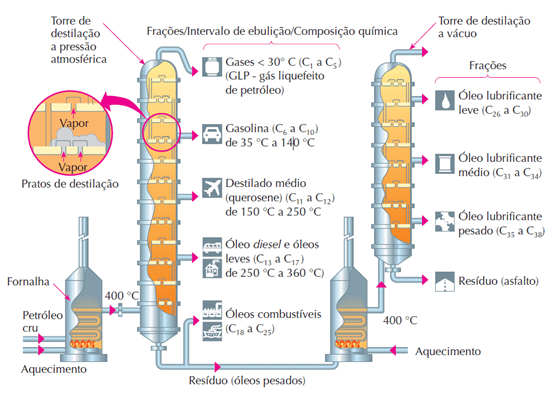
\includegraphics[scale=0.4]{../img/petroleo2.png}
\end{center}
\end{block}
\end{frame}
\begin{frame}[label={sec:orgd0183e3}]{Cromatografia}
\begin{block}{Cromatografia}
Processo de separação utilizado quando existem pequenas quantidades de amostras da mistura e das substâncias que a constituem têm diferentes capacidades de absorver num material sólido. \alert{Misturas homogêneas}

\begin{center}
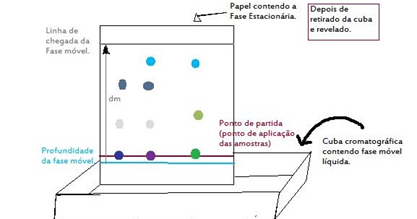
\includegraphics[width=.9\linewidth]{../img/cromatografia2.png}
\end{center}
\end{block}
\end{frame}
\begin{frame}[label={sec:org61f8f64}]{Liquefação Fracionada}
\begin{block}{Liquefação Fracionada}
É o método utilizado para fracionar os componentes gasosos presentes em uma mistura gasosa que é resfriada e comprimida até que todos os componentes sofram liquefação. A seguir, a mistura líquida e homogênea é destilada e as substâncias gasosas são obtidas separadamente. Essa técnica é muito utilizada para obter nitrogênio e argônio a partir do ar atmosférico.

\begin{center}
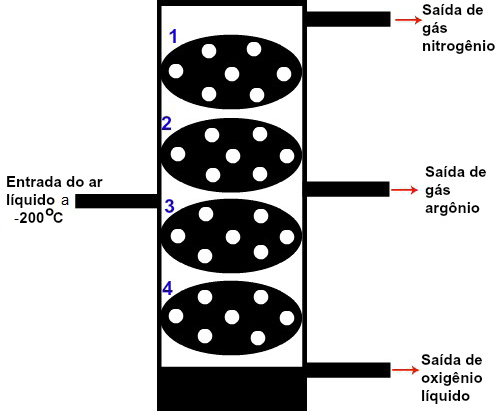
\includegraphics[scale=0.38]{../img/liquefacao_fracionada.png}
\end{center}
\end{block}
\end{frame}
\begin{frame}[label={sec:orgbc093dc}]{Aplicação}
\begin{block}{Tratamento de Água}
\begin{description}
\item[{Coagulação}] É quando a água bruta recebe, logo ao entrar na estação de tratamento, uma dosagem de sulfato de alumínio. Este elemento faz com que as partículas de sujeira iniciem um processo de união.
\item[{Floculação}] Quando, em tanques, continua o processo de união das impurezas, na água em movimento. As partículas se transformam em flocos de sujeira.
\item[{Decantação}] As impurezas, que se aglutinaram e formaram flocos, vão se separar da água pela ação da gravidade, indo para o fundo dos tanques ou ficando presas em suas paredes.
\item[{Filtração}] A água passa por grandes filtros com granulações diversas e carvão antracitoso (carvão mineral). Aí ficarão retidas as impurezas que passaram pelas fases anteriores.
\item[{Desinfecção}] É a cloração, para eliminar germes nocivos à saúde e garantir a qualidade da água até a torneira do consumidor. Nesse processo pode ser usado o hipoclorito de sódio, cloro gasoso ou dióxido de cloro.
\item[{Fluoretação}] É quando será adicionado fluossilicato de sódio ou ácido fluorssilícico em dosagens adequadas. A função disso é prevenir e reduzir a incidência de cárie dentária, especialmente nos consumidores de zero a 14 anos de idade, período de formação dos dentes.
\item[{Correção}] É a correção de pH, quando é adicionado carbonato de sódio para uma neutralização adequada à proteção da tubulação da rede e da residência dos usuários e não haver corrosões.
\end{description}

\begin{center}
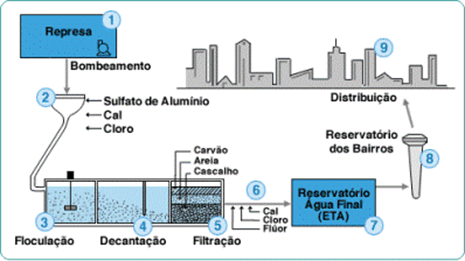
\includegraphics[width=.9\linewidth]{../img/estacao_agua.png}
\end{center}
\end{block}
\begin{block}{Tratamento de Esgoto}
O principal método de tratamento de esgoto e efluentes é o do lodo ativado, que consiste na degradação dos materiais orgânicos por bactérias aeróbias.


\begin{description}
\item[{Peneiramento ou gradeamento}] O esgoto passa por grades ou peneiras para retenção de sólidos grandes;
\item[{Caixa de areia}] Aqui as areias, mais densas, são separadas do esgoto por decantação;
\item[{Decantação primária}] Em um decantador primário ocorre a sedimentação das outras partículas sólidas presentes;
\item[{Aeração}] Nos tanques de aeração, é inserido ar próximo à entrada de esgoto, fazendo multiplicar os micro-organismos presentes no esgoto, para que degradem o material orgânico através de seu metabolismo natural;
\item[{Decantação secundária}] Após a aeração, o efluente tratado é separado do lodo ativado, que é coagulado e decantado para o fundo do tanque. Parte deste lodo é retornado ao tanque de aeração para contribuir com a degradação das impurezas e o restante é separado para secagem e descarte apropriado. A água resultante pode ser descartada em um corpo hídrico ou reutilizada.
\end{description}

\begin{center}
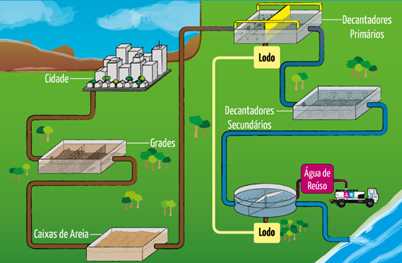
\includegraphics[scale=0.7]{../img/estacao_esgoto.png}
\end{center}
\end{block}
\begin{block}{Fim da Aula}
\begin{tikzpicture}
\node[graduate,sword, devil, minimum size=1cm]{ \bfseries Bons Estudos !!!!};
\end{tikzpicture}
\begin{center}
\begin{tabular}{ccc}
Download Aula & Resumo & Lista de Exercícios \\
 \qrcode[height=1.5in]{https://github.com/fabinholima/AulaQuimicaPDF/blob/main/QG/SeparacaoMisturas/Separacao_Misturas.pdf} & \qrcode[height=1.5in]{https://github.com/fabinholima/AulaQuimicaPDF/blob/main/QG/SeparacaoMisturas/Resumo_SeparacaoMisturas.pdf}& \qrcode[height=1.5in]{https://github.com/fabinholima/AulaQuimicaPDF/blob/main/QG/SeparacaoMisturas/Lista_SeparacaoMisturas.pdf}\\
 \end{tabular}
 \end{center}
\end{block}
\end{frame}
\end{document}
